\chapter{Cluster-Based Visualization Design for Merger Tree Data}

%NOTE: convince the audience that this is a very common problem that limits the types of things that we can use clustering for!

% can talk about the scatter plot experiments, and the progenitor-drawing experiments, to convince that we've explored a big chunk of the possible design space

% big simulations are common; visualization can help analyze them, but it's hard at increasing scales.
Across domains such as astrophysics, atmospheric science, particle physics, and fluid dynamics, scientists are using growing computing power to create increasingly high-resolution simulations~\cite{hacc},~\cite{Steed:2013:BDV:2538033.2538071}. Simulated models of physical systems allow scientists to perform a range of important tasks: explore how external variables affect physical systems, compare simulated and observed data, and project outcomes. Visual analysis can be an important tool for understanding such simulations, but increasing data size and dimensionality challenge traditional visualization approaches with clutter, obstruction, and overburdened visual channels~\cite{taxonomy_clutter_reduction}. %^ this paper notes that the problem is worse for unstructured exploration, as opposed to investigating something in particular

% clustering is one approach. here are a bunch of examples that establish the scope.

%visualizations that use clustering.
A common solution is to aggregate simulation data, then visualize information about the resulting groups. Clustering is applicable to a wide range of data---it primarily requires defining the ``similarity'' between any two data points---and often, clusters have a natural, scientifically significant meaning. The process can help categorize physical phenomena and characterize overall trends. Visualization researchers have applied clustering to a wide range of applications (see Section~\ref{relatedwork}). Outliers can be exposed in the clustering process; these outliers may indicate interesting scientific phenomena or problematic simulation code. Approaches such as hierarchical clustering allow for intuitive multi-resolution exploration so that scientists can understand trends and outliers at many levels of detail. 

% but, clustering abstracts the data, partly because of the black box, and also we're a bit in the dark because the above examples don't really validate whether the clustered results are helpful.
However, clustering abstracts the underlying data into information about groups of the data. This abstraction is a loss of information about outliers, noise, subtle differences between time series, and data-processing steps. Growing data sizes magnify the threats from abstraction, because more data are being represented per visual element.  The ``black box''---or unseen inner workings---of a clustering algorithm is another significant source of the threat from abstraction. 

%There are few visualization efforts to show information to the user about how the clusters were generated. (TRUE?/CITE EXAMPLES)
%The visualizations of clustered data listed above do not depict the process of deriving clusters from the data. [this is hard to depict - CITE - ?]
% IMPORTANT: would be good to show through the examples that clustering isn't necessarily the only solution here, but abstraction in some sense always has to happen

% at least in those examples, though, there are often expectations for clusters/natural groupings. some data, like ___ or merger trees (see section __), don't have natural groupings but face a big data/vis problem. 
In some cases (see Section~\ref{relatedwork}), expectations for the groupings can help users make sense of a clustered visualization despite the abstraction and black box, which provides some validation. However, there may be only vague expectations for trends and groupings within simulation data. This is the case for simulated dark matter merger trees (see Section~\ref{background}). We explore a clustering visualization approach for merger trees from N-body simulations. We propose that, for a clustered, abstracted representation to enable useful visual analysis of these data, we should provide flexible clustering options, linked multidimensional views, and information about the black box. 

%In our preliminary survey, this limited scientists when interpreting visualizations of clustered merger tree data. % be more explicit about 'confused' 

% here, we see if we can address this problem (for one case) by 1) providing strongly multidimensional and controllable clustering vis and 2) showing the black box 

In this work, we develop the following to enable more meaningful representation and exploration of merger tree data:  

\begin{itemize}
\item{Problem characterization and abstraction~\cite{trenches_stacks} for analyzing dark matter merger trees.}
\item{An extension of the contour boxplot~\cite{contour_boxplot} for groups of multivariate time series, which enables visualizing groups of unconventional data structures like trees.}
\item{A flexible clustering approach to support free-form exploration and user-defined centroids.}
\item{A visualization approach for understanding the pairing process in a clustering algorithm.}
% FUTURE: \item{A reflection on existing design guidelines in the context of this application's particular challenges.}
\end{itemize}

%%%%% BACKGROUND %%%%%

% sum up why merger trees are a particularly hard domain, and sell that addressing the problems for it is a good pursuit.

\section{Analyzing Dark Matter Merger Trees}
\label{background}

% what are merger trees and why should we care?
Scientists use simulation frameworks such as Illustris~\cite{illustris_info} and HACC~\cite{hacc} to study how dark matter forms its structure in the universe. The simplest approach is an N-body simulation: initially, dark matter ``particles'' are distributed throughout a volume. The gravitational attraction among particles creates dark matter ``halos'' that merge into one another to become increasingly large halos. Each halo present in the final timestep can be characterized by its history: which halos merged together to form this particular dark matter clump, and when? The plots of these halo histories, actively studied in cosmology research, are called ``merger trees'' (see Figure~\ref{diagram}).

One reason to study halos and merger trees is that galaxies, which contain the majority of their mass in dark matter, form within halos. Merger trees may help explain the connection among dark matter halos, their environments, and how galaxies form within them. For an in-depth discussion of dark matter halos, merger trees, and galaxy formation, see~\cite{lacey1992}.

% what is the workflow/scientific process for analyzing merger trees?
	% how do they find outliers?  
    % for good analysis, one needs to be able to see all the data, identify trends & different types of outliers
Through literature review and a survey of several researchers studying merger trees in N-body simulations, we identified tasks and guiding questions for analyzing dark matter merger trees~\cite{hacc},~\cite{masshistory},~\cite{lacey1992}. We also proposed the idea of clustering trees into groups and solicited questions about that approach.
\begin{itemize}
\item{Do halo properties, e.g., \textit{concentration} or \textit{formation time}, correlate with characteristics of their merger trees?} %‘in what sense is concentration a classifier of histories?’%}
\item{Can we identify anomalies such as missed progenitors or heavy births (i.e., instances where the sum of progenitor masses does not explain a halo's mass, or where a new halo is identified by a halo finding algorithm that was not present in previous timesteps)?}
\item{When, and why, do anomalies in the simulation appear?} %note for later: this needs a system like our previous one to be investigated, but that system needs a complement (This system) to facilitate actually finding the outlier trees.
\item{How many outlier and non-outlier merger trees are there?}
\item{What is the measure of similarity between trees for forming the clusters?}
\end{itemize}

% ... clustering can potentially answer these questions because ____.
Done correctly, clustering may be a scientifically meaningful approach to visualizing merger trees that could address the above questions. Most trees likely follow only a few different types of mass histories throughout their lifetimes~\cite{masshistory}, meaning they can naturally be grouped into clusters that describe these patterns. Outliers, which might represent a unique physical phenomenon or a code bug, can be placed alone or in smaller clusters if the similarity metric singles them out (see Section~\ref{clustering}). A cluster-based visualization for merger trees may be successful, then, if the similarity metric identifies meaningful, non-arbitrary groupings and outliers, and if the properties of the resulting clusters are intuitive to viewers.

%mention somewhere?, that in the preliminary survey, they didn't really know how to answer 'do these clusters meet your expectations'

%establish why we need vis (finding patterns and outliers can be enabled by visualization. 
	% some things (that we're looking for) can be identified analytically but we also don't know what we're looking for
%(galaxy formation is poorly understood; CITE)
    
\section{Related Work}
\label{relatedwork}
One motivation for this study is that existing tools to study ensembles of merger trees are quite limited. Simulations can yield millions of merger trees. Researchers have most often visualized merger trees by rendering each node and edge, such as in~\cite{scivis15},~\cite{Shan:2014} (Figure~\ref{node_edge}). This approach cannot accommodate all output from a simulation. Rendering all merger trees at once prevents scientists from discerning global patterns or individual discrepancies~\cite{ellis2007},~\cite{elmqvist2010}; occlusion from over-plotting particularly affects the many low-mass halos. 

\begin{figure}[h!]
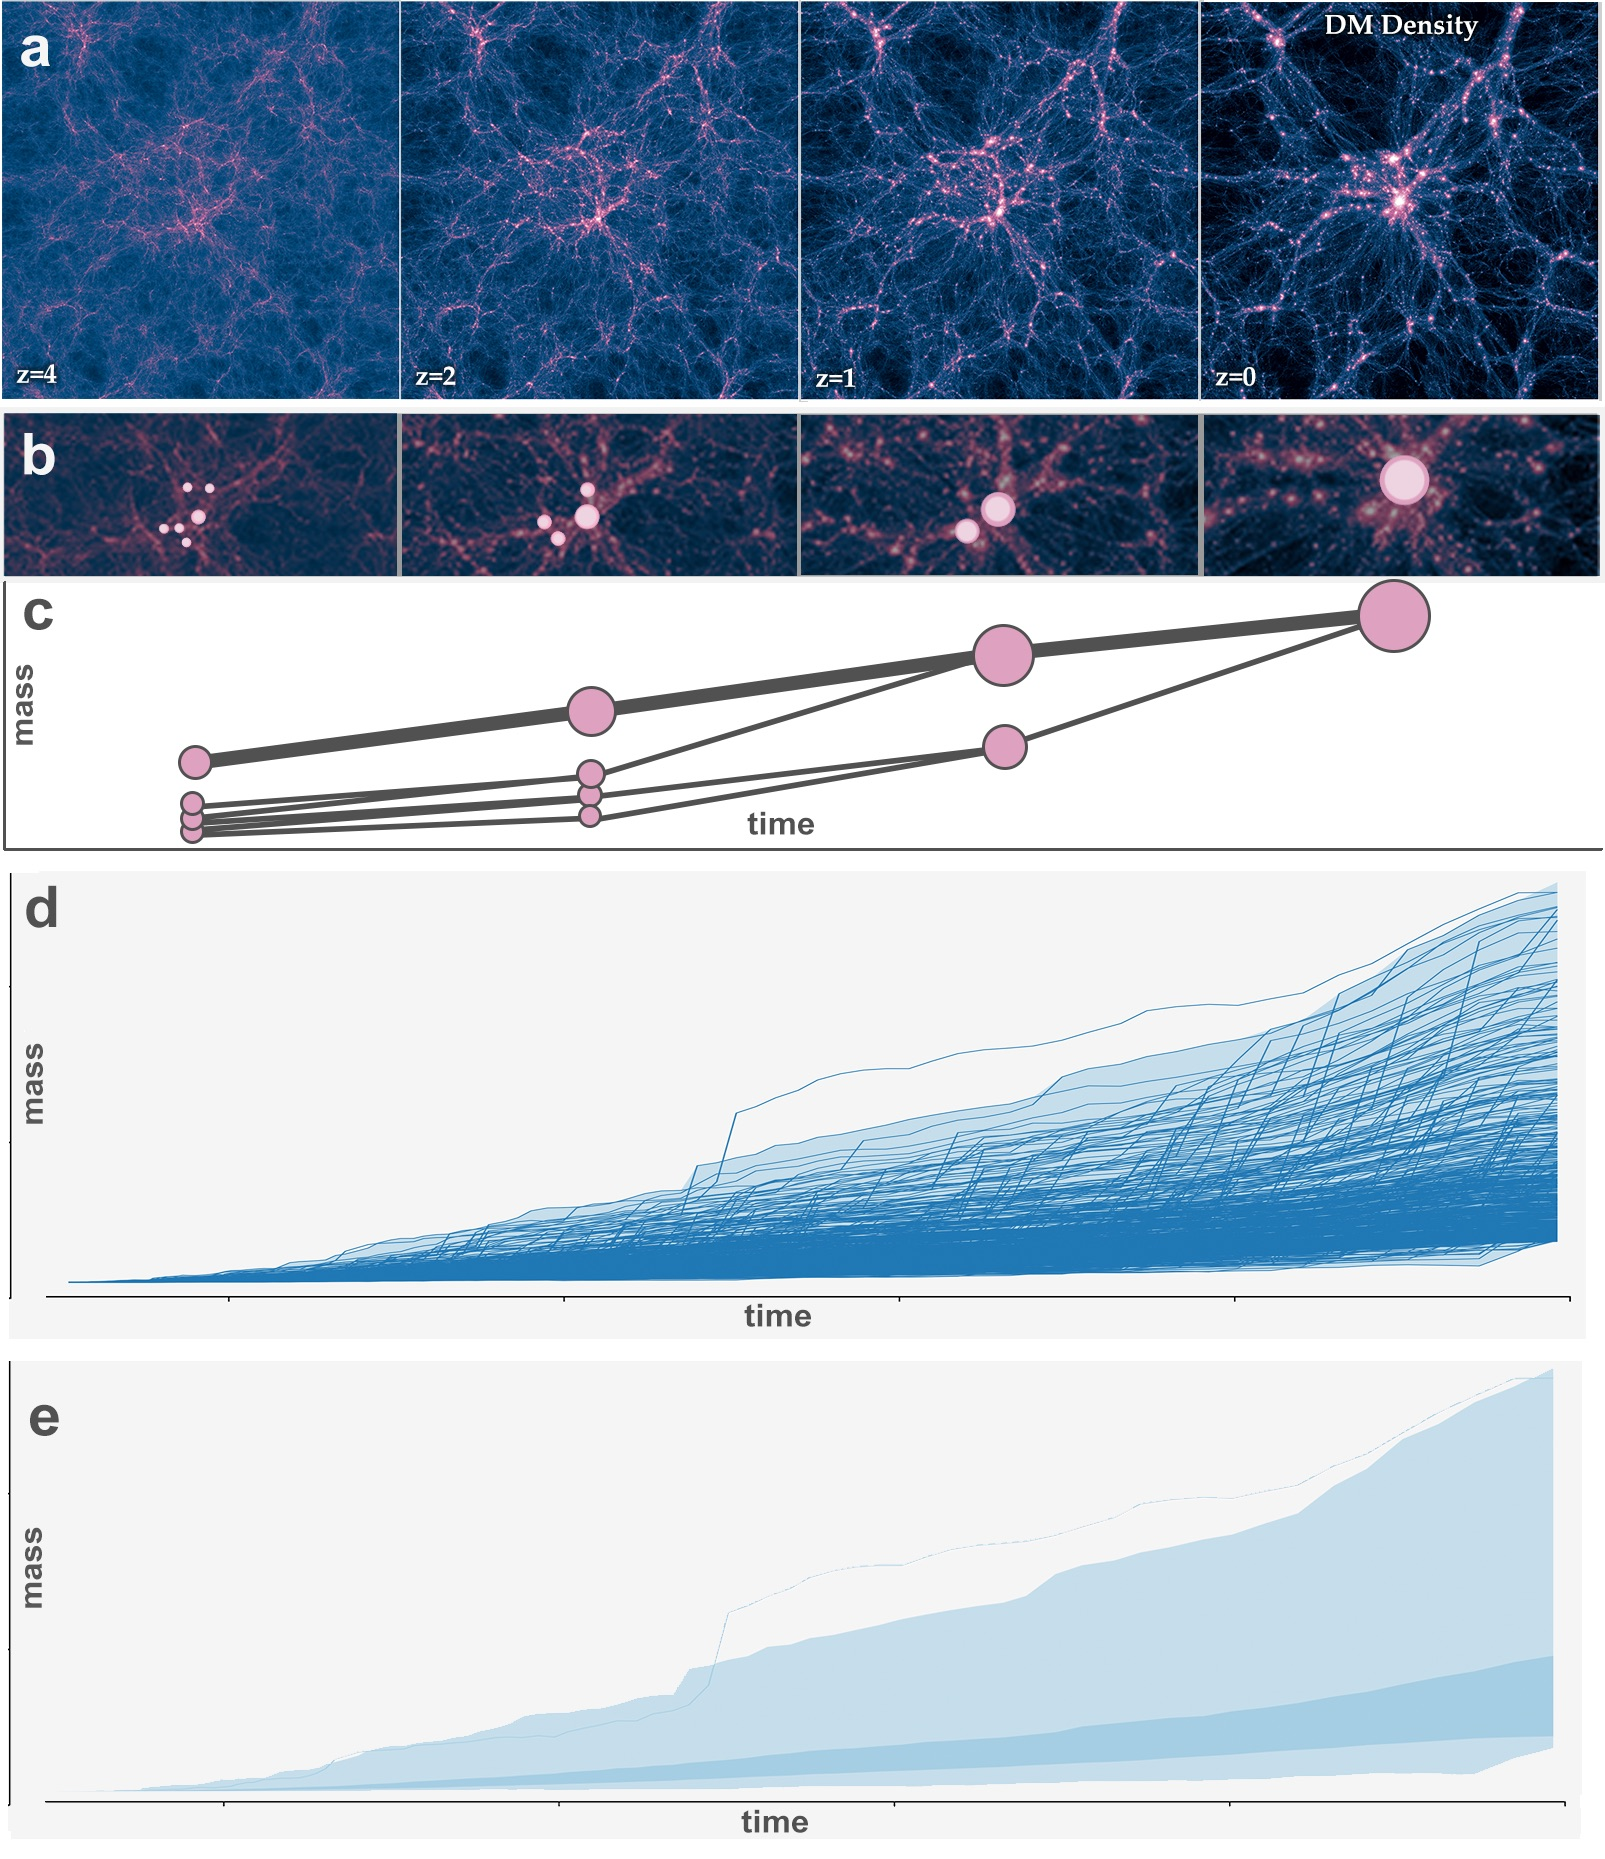
\includegraphics[width=\textwidth]{images/clusters/particles_to_tree_cluster.jpg}
\caption{The process of abstracting dark matter simulation data (a) into clusters of merger trees (e). For each timestep of the simulation, dark matter halos are identified using a halo finding algorithm (b). Here, we show four timesteps of the Illustris simulation (a) (Image credit: Illustris Collaboration). In (b), we highlight the progenitor halos for the single halo in the final timestep on the far right. A simple merger tree (c) shows how halos merge together in each timestep. The ``main branch'' is highlighted. In (d), we show all main branches, over all timesteps, for one mass bin. We represent clustered main branches by their range of values, with the middle $50\%$ highlighted and an outlier rendered separately (e).}
\label{diagram}
\end{figure}

\begin{figure}[h!]
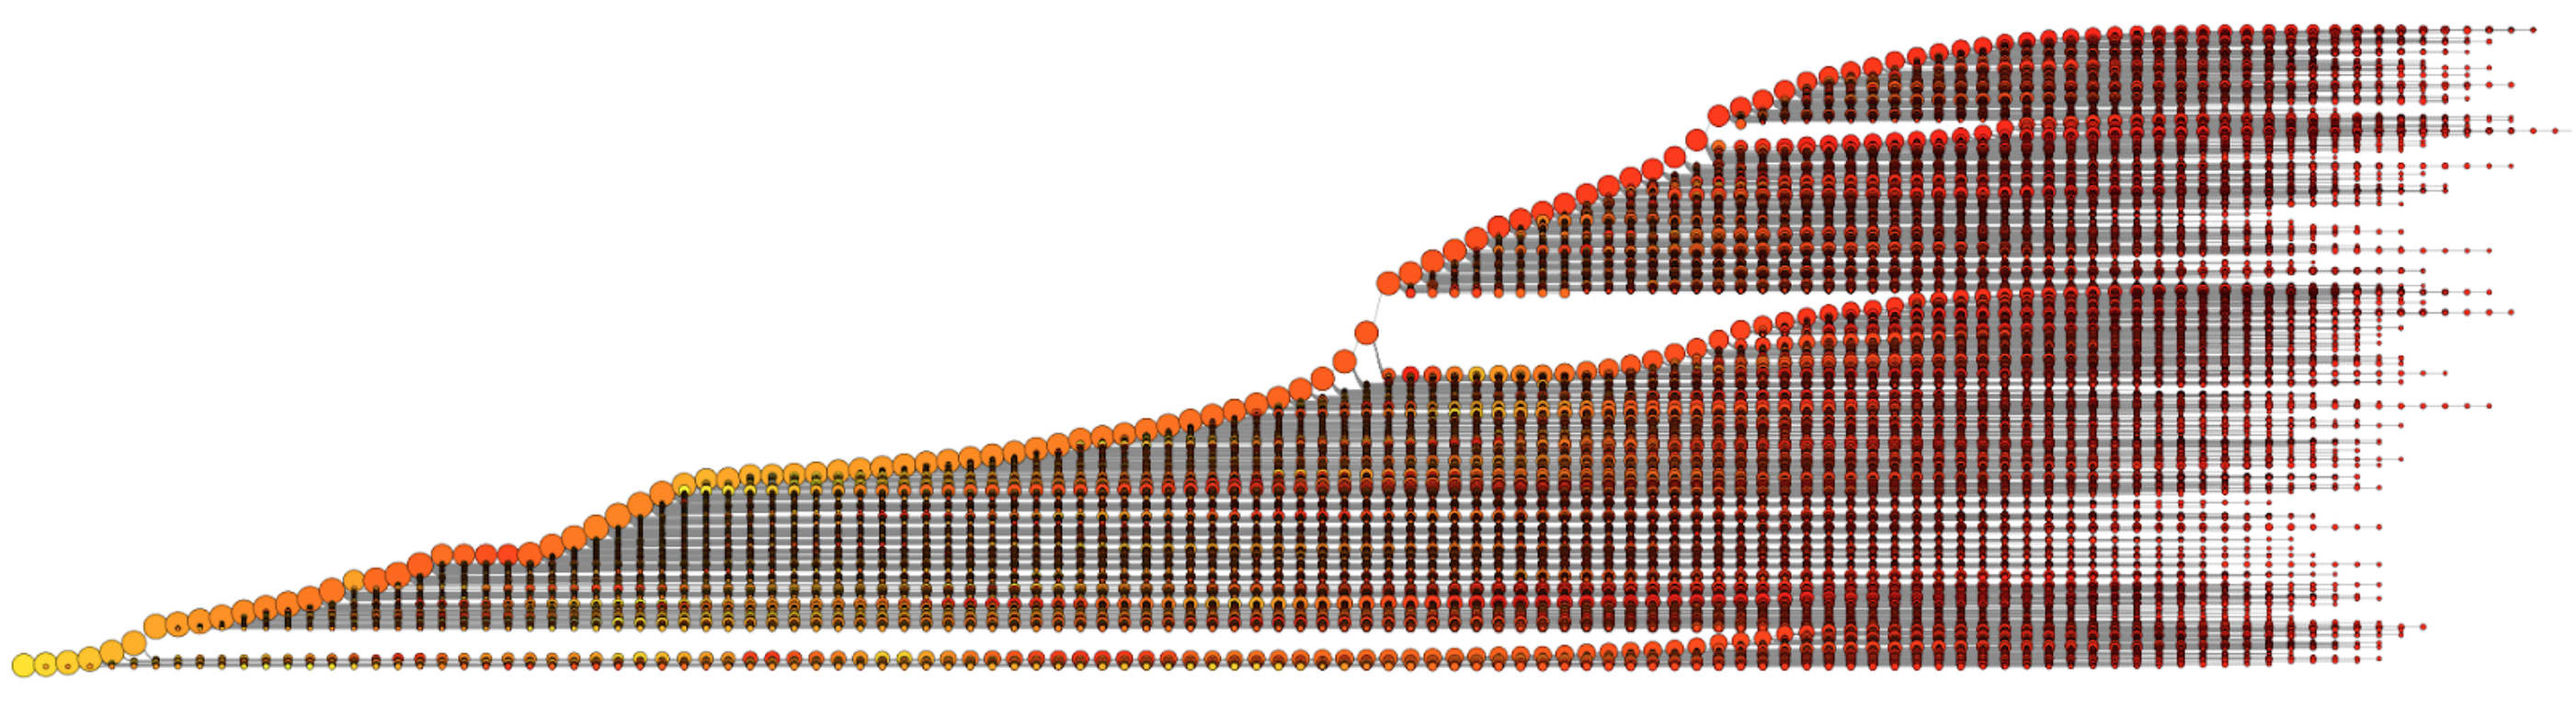
\includegraphics[width=\textwidth]{images/clusters/illustris_tool}
\caption{A snapshot from the Illustris Merger Tree Tool (credit: Illustris Collaboration). The halo masses are mapped to the circles' sizes, and velocity is mapped to color. This approach can show complex progenitor behavior for a single merger tree.}
\label{node_edge}
\end{figure}

Zooming and panning cannot provide clarity, because viewing segments of merger trees very close-up removes context and time-varying trends. %what analysis goes with this? why is it useful sometimes but why is it hard? T
There are also 3D visualization approaches showing the spatial position of each halo throughout the merging history, such as in~\cite{7429496}. %later -- and FIND THIS CITATION. 

% why don't we have expectations for the trends? (cite survey of scientists that we did.)

%clustering applied to scientific data in general.
In general, clustering has been used to help visualize a variety of scientific data. The authors of~\cite{k-means--} create a version of \textit{k}-means with enhanced outlier detection and test it on a set of hurricane trajectories. The outliers identified are not compared to the non-outliers and do not seem to have clear reasons for being outliers.

%~~~~
The authors of~\cite{wei2012} propose a fast, scalable clustering technique for multi-length data from combustion simulations that allows the clusters to be subject to users’ specifications. However, this approach for visualizing particle paths lacks scalability: it uses sight-based outlier rejection, which requires that only a small number of particle trajectories are rendered at once. It is unclear how to make sense of a larger dataset or a larger group of clusters. Another approach, explored in~\cite{hier_parallel}, uses a parallel coordinates representation with gradiated bands to visualize aggregated data. Parallel coordinates can also be used in a focus + context visualization in a way that preserves outliers~\cite{outlier_parallel_coords}. The authors of~\cite{group_dynamics} create a group feature tracking framework for scientific data which is shown to be effective on turbulent flow data; this work does not focus on scientific usefulness or on specific use cases. 

A unique approach in~\cite{weather_ensembles} aggregates ensembles of weather forecasts, visualizing when and how various forecasts diverge. In~\cite{ocean_models}, the authors develop a specialized approach for aggregating ocean model data based on clustering ensembles, allowing scientists to compare simulation output with observations. The work in~\cite{relevant_parts} establishes an interactive visualization method for defining relevant parts of trajectories in 3D space and interactively refining the clustering. Finally, the clustergram~\cite{clustergram} is a scalable clustering visualization method that can show how items are added to clusters; this could be useful for opening up the “black box” of clustering to end users.

%~~~~~~

\begin{figure*}[h]
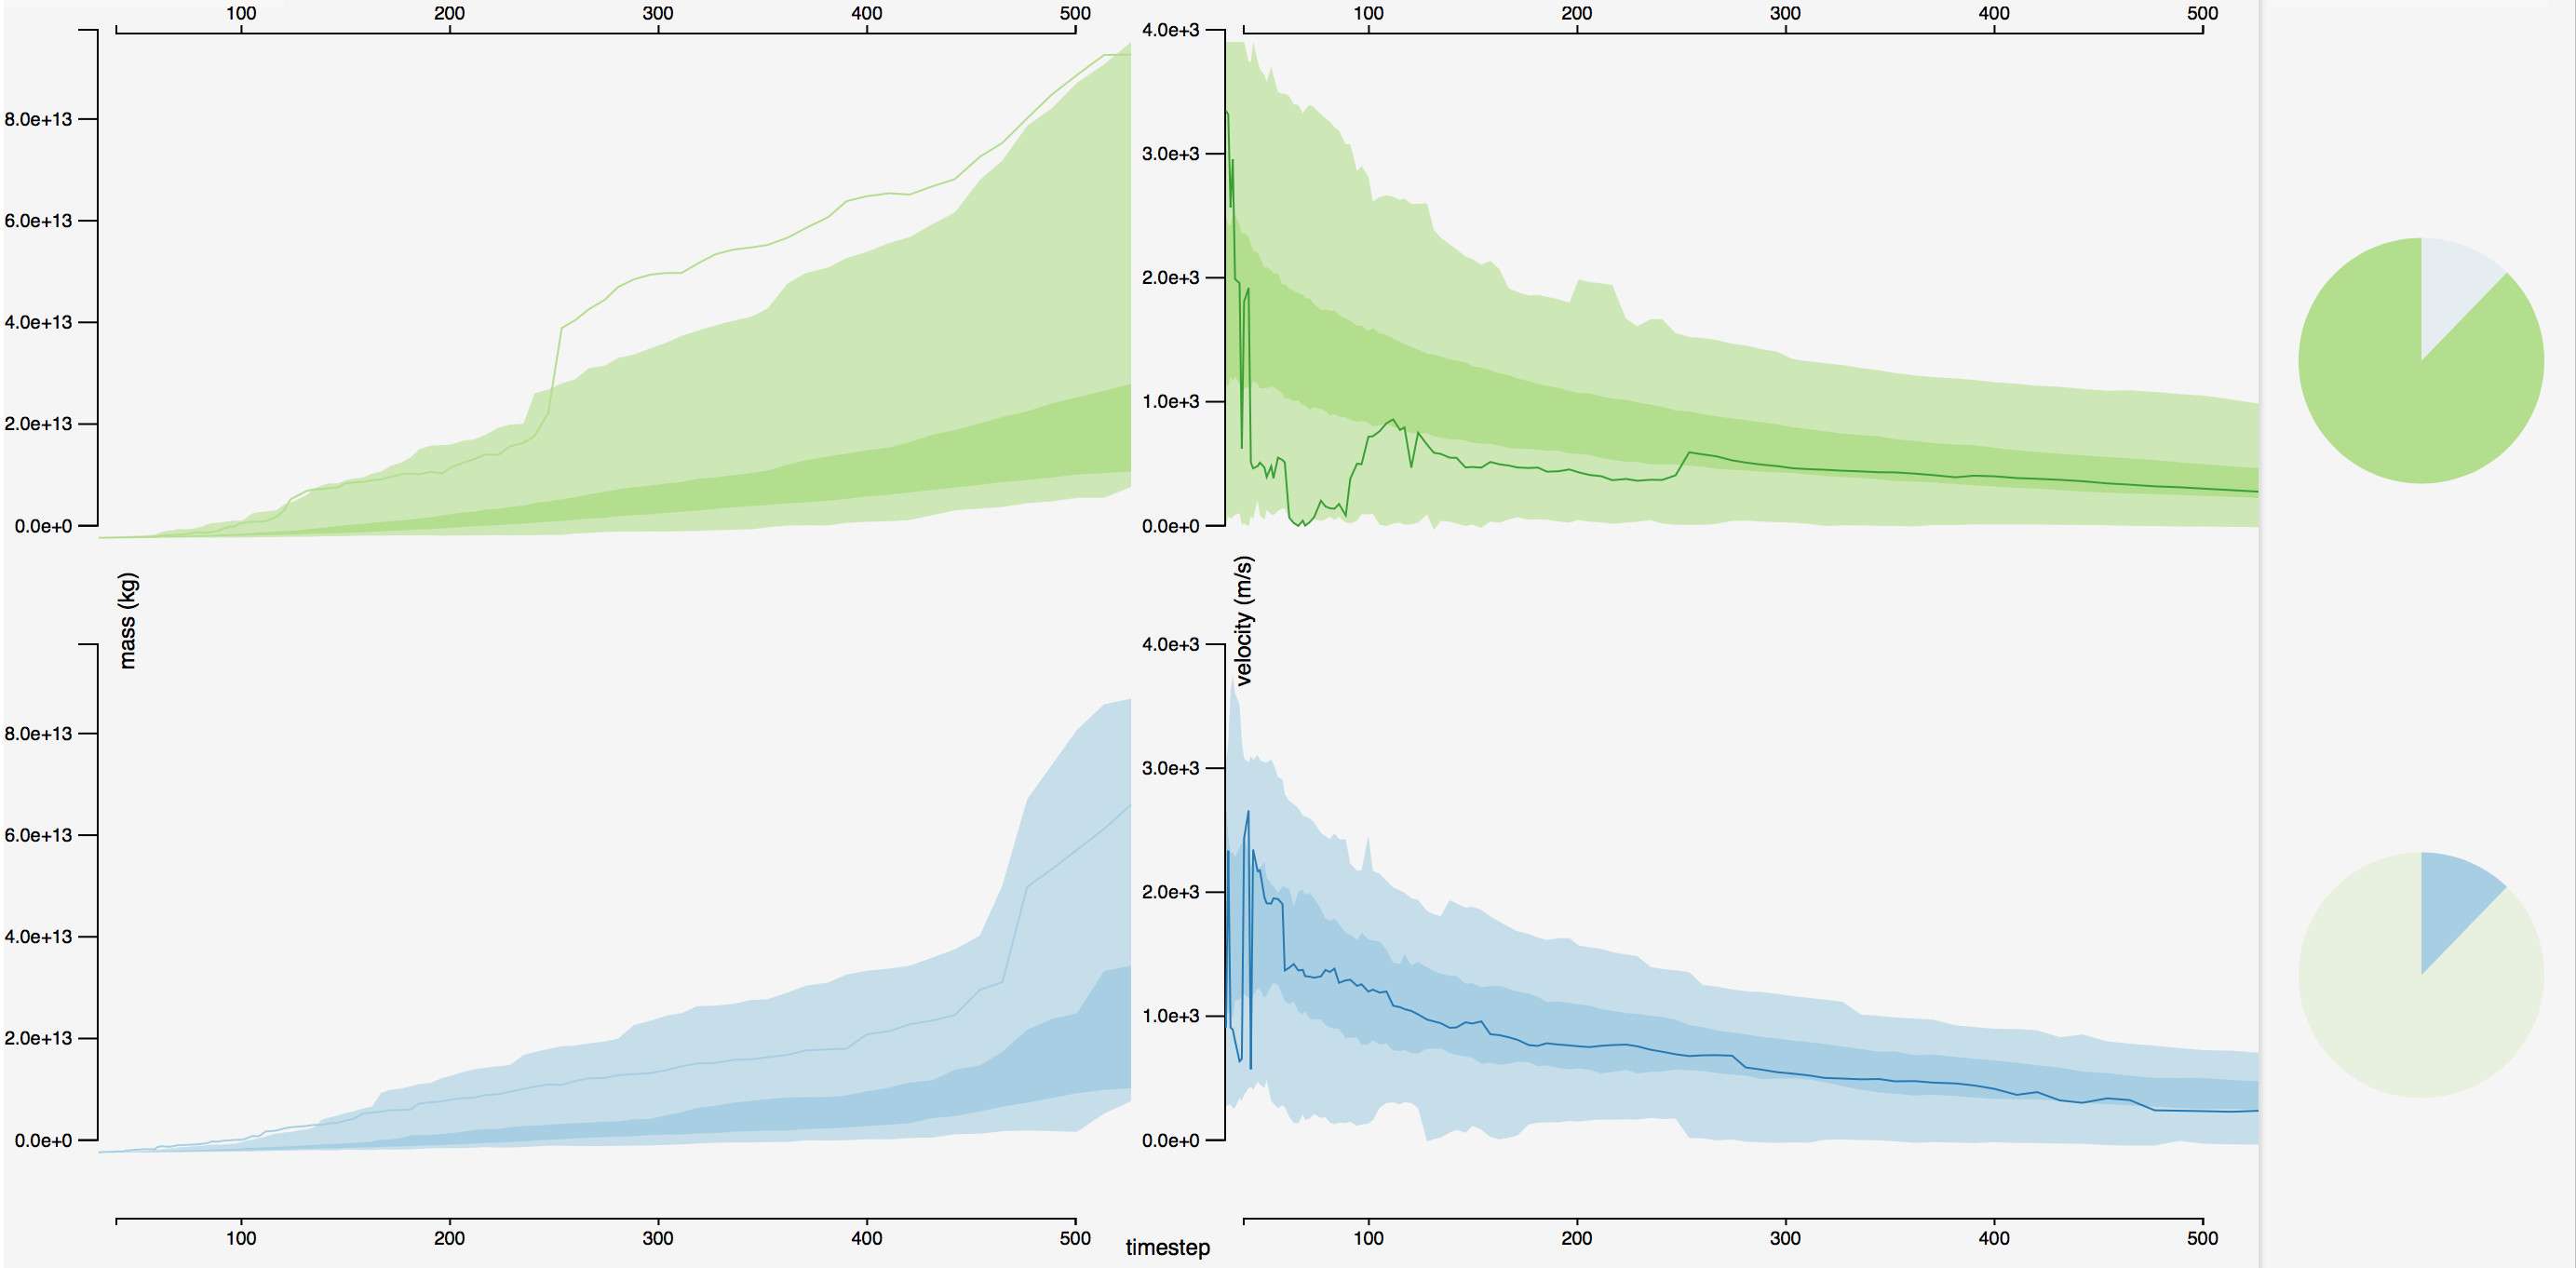
\includegraphics[width=\textwidth]{images/clusters/n2_mass_velocity_outliers}
\caption{Mass (left) and velocity (right) for a single mass bin with $n_{\mathrm{clusters}}=2$. Outliers are highlighted in each view (the outlier is the same tree for the mass view and the velocity view). While the blue outlier seems similar to the rest of its cluster, the green outlier merits further exploration. It has an unusually low mass for the first half of the simulation, then experiences a large mass increase and a sudden velocity shift around $t=250$.}
\label{vel_example}
\end{figure*}

%%%%% METHODS %%%%%

\section{Design Decisions}
%* identify threats (abstraction, distrust) for each choice

%* couch this in terms of existing design guidelines, as mentioned by pvast reviewer

We use data from a run of HACC~\cite{hacc} that yielded about four million merger trees, each including thousands of data points with position, velocity and mass. Based on our preliminary survey, we choose to group the merger trees by binning their root masses; this is a common approach~\cite{masshistory},~\cite{assemblyhistory}.
%(can leave out:)
%(explain?)

\begin{figure}[h]
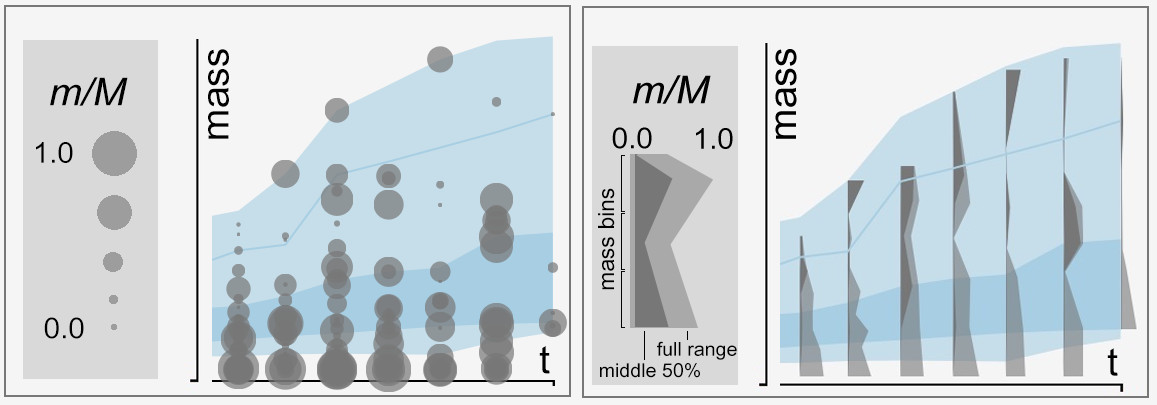
\includegraphics[width=\textwidth]{images/clusters/merger_abstraction_diagram}
\caption{How we abstract merger data in our approach. On the left, a circle for each merger represents the merger ratio $m/M$, i.e., the ratio of progenitors to the main branch halo being merged into. Low-mass halos clutter this representation. On the right, we use a modified violin plot to represent the range of merger ratios (horizontal axis) for each mass bin (vertical axis) at each timestep.}
\label{merger_abstraction}
\end{figure}

\subsection{Defining Clusters}
\label{clustering}
%better DTW example image, with real data (i.e. in our view)

%overall: mass is a baseline because it's the most intuitive/common thing to go with
% Many data clustering algorithms were designed for numerical data~\cite{clusteringbook}, in contrast to continuous data common in scientific simulation outputs such as mass and velocity.  %therefore, ...?
% ^^ PUT THIS IN FULL VERSION. /quals.
% there's a lot of info for clustering to abstract away
For visual analysis in general, data science approaches like clustering are best for ``crisply defined tasks''~\cite{trenches_stacks}, rather than the broad exploratory questions considered in this study.
%therefore?
Additional challenges include that merger trees have varying lengths in time, and that mass and velocity values can differ by nearly an order of magnitude. 
% and of course, no ‘natural’ clusters or subsetting; only a few percent might be interesting; 

% dist metric: want the clustering to be based on scientifically/physically significant similarities/differences
Clustering data requires a “distance metric” that measures the relative similarity of data points, i.e., the similarity of two merger trees. In our case, this metric depends on a set of features representing each merger tree. To choose these, we can use \textit{feature extraction} or \textit{feature selection}. Feature extraction includes techniques like Principal Component Analysis~\cite{clusteringbook}, which warp data into a lower-dimensional representation by combining parameters. Feature selection, instead, uses a set of existing attributes---in our case, mass, velocity, number of mergers, etc.---to characterize data.

% NOTE: here, doing feature selection, we explore the design space ~of the existing parameters~. this gets us pretty far because we can see that mergers are really important while velocity (and spatial position) are not that telling. if we use feature extraction, we can explore a much larger space of options, like combined effects of two variables.

Feature selection has an intuitive interpretation, while feature extraction yields more complex features that may have greater predictive power but a more arbitrary meaning~\cite{clusteringbook}. Both approaches can contribute to abstraction by masking the data's underlying properties. To reduce abstraction, we use the most common approach in cosmology research: feature selection using the main branch mass representation~\cite{masshistory},~\cite{assemblyhistory}. This decision eliminates clutter by removing low-mass halos, which have relatively small effects on their merger trees and are often omitted from analysis.

We choose Dynamic Time Warping (DTW)~\cite{clusteringbook} to calculate the distance between each pair of main branches. DTW accommodates time series of different lengths and with inconsistent sampling frequencies, such as merger trees. It calculates how much one time series would have to warp in order to match another time series. A pair of merger trees can be ranked as similar if they share main branch features shifted by some time phase. 

%%FIGURE
\begin{figure*}[h]
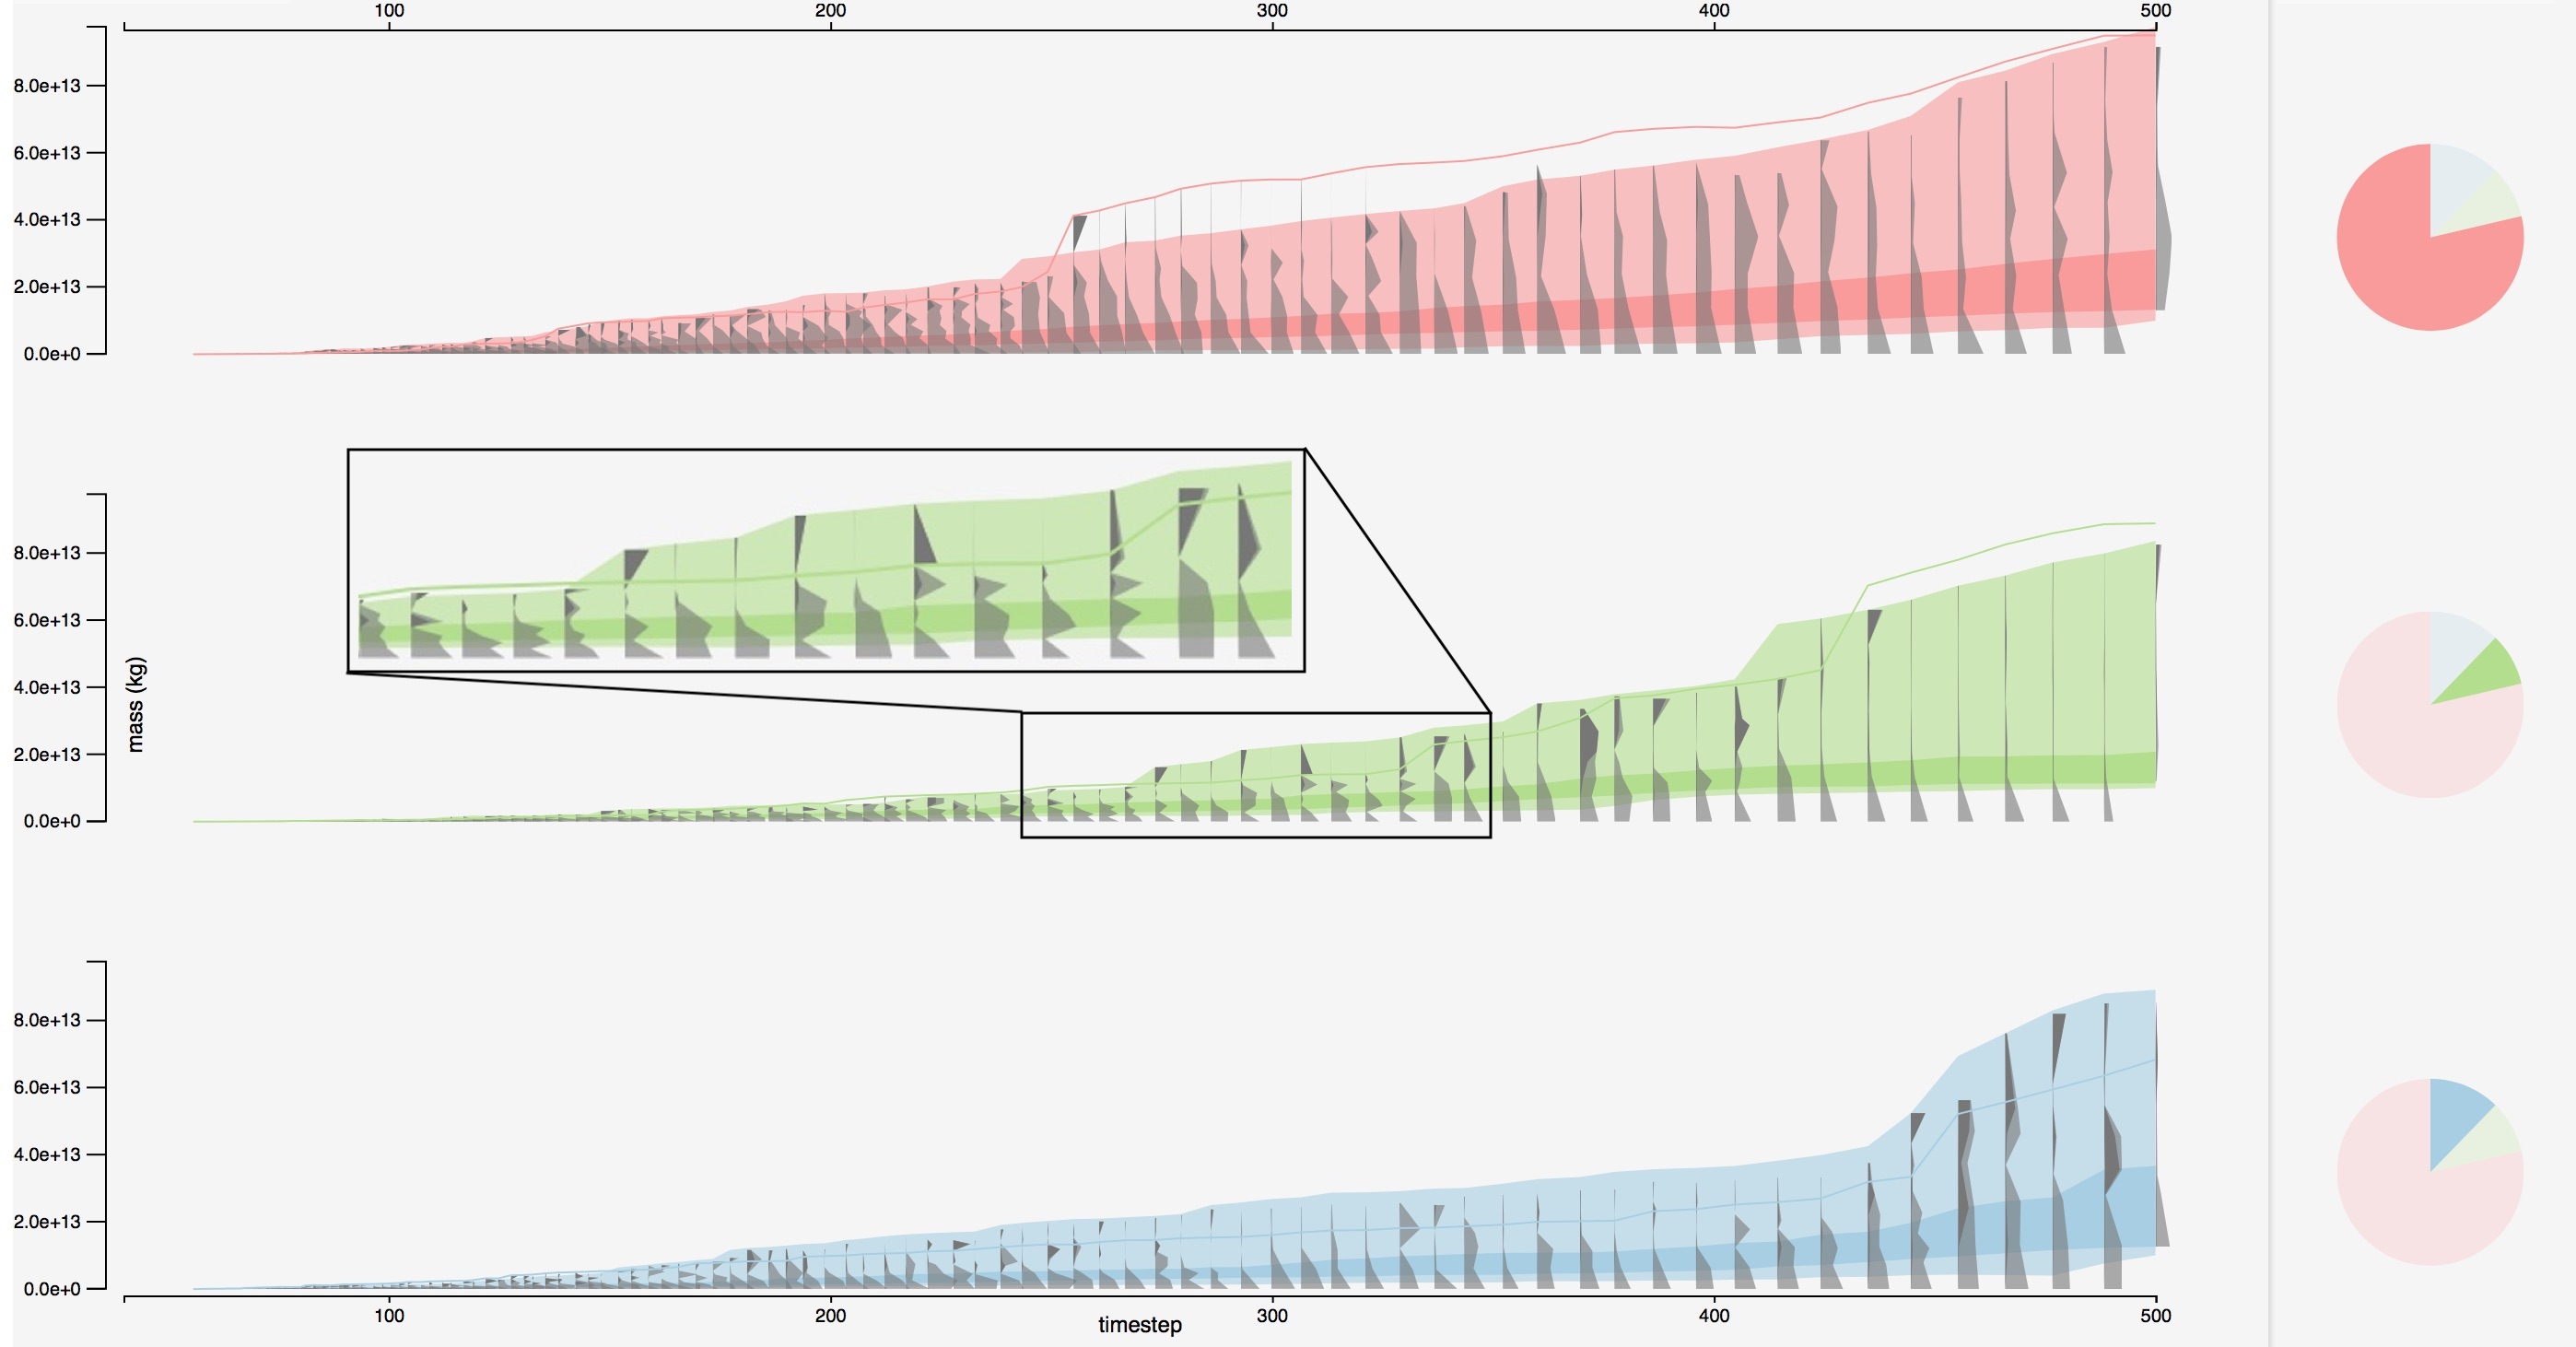
\includegraphics[width=\textwidth]{images/clusters/n3_d0_with_mergers}
\caption{Merger trees for one mass bin ($10^{13}\mathrm{kg} < M < 10^{14}\mathrm{kg}$), divided into three clusters based on DTW similarity for main branch mass. The colored shapes show the distribution of main branch masses over time, while the gray shapes show distinct merger activity for each cluster (see Figure~\ref{merger_abstraction}). One outlier per cluster is rendered with an individual line. At right, pie charts show the relative proportion of trees in each cluster.}
\label{three_clusters_with_mergers}
\end{figure*}

%linkage: unclear; difficult to visualize; we offer the choice because \shrug and this doesn't bias them too much at least hopefully
We also need to define the similarity between two groups of main branches. This option is known as ``linkage.'' Three common linkages are \textit{single}, \textit{complete}, and \textit{average}~\cite{clusteringbook}. Linkage significantly affects clustering results. Single linkage has the tendency to form ``long chains,'' adding most members to one cluster while leaving outliers unpaired. These clusters might contain quite disparate main branches, but the outliers left exposed should be even more disparate. Complete linkage tends to form clusters with more consistent characteristics and sizes [42], perhaps yielding better summaries of the data set.
In this step, we may be trying to group data that do not necessarily fit neatly into categories. However, we find that average or complete linkage is useful for characterizing merger trees, while single linkage better distinguishes outliers (see video).

At each step in the algorithm, the two merger trees or groups with the smallest distance are grouped; this creates a hierarchy of clusters. We can query the hierarchy at any level to return the desired number of merger tree groups. These DTW-generated groupings provide the default for our visualization. However, to provide more flexibility, we allow users to pick a tree as a centroid around which to re-cluster the data.  For now, we only implement $n=2$ as a proof of concept. Therefore, for each new centroid, we only have to check the distance matrix once to find the maximally distant tree, define that tree as the other centroid, and then define clusters based on the nearest centroid. These results can address our scientific goals: scientists are interested in how many outliers of each type there may be, and how much they diverge from other trees.
This approach can be further improved, such as narrowing the neighborhood around the target centroid in order to get more precise groupings.
%(see supplemental video!)

%%%%% VISUAL ENCODING %%%%%
%...these are the choices, and this is how they abstract the data.

\subsection{Visual Encoding}
%challenge: we're visualizing a pretty abstracted set of data; 
	% inconsistent number of data points per timestep per series, so hard to depict distributions of distributions
    
% 0th: overall guidelines we'll try to follow:
First, we establish design guidelines: the authors of~\cite{Albers:2014:TEA:2556288.2557200} suggest that color is best for ``summary comparisons,'' especially when the aggregation is not explicit, and that position is best for ``point comparisons,'' i.e., comparing individual data points. We use color to indicate categories, designating a color family for each cluster. We use position for comparison among clusters, providing a common baseline of a quantity vs. time, as suggested in~\cite{graphical_perception}.

% SAY THAT WE SHOW DTW PAIRS IN THE VIDEO.

\subsubsection{Clusters and Merger Trees}
%first, how to make the visual aggregates:
%contour boxplot to show distributions of paths; 
One framework for visualizing aggregated data~\cite{elmqvist2010} suggests creating \textit{visual data items,} i.e., single merger trees, and \textit{visual aggregates,} i.e., clusters. These aggregates should describe the data points within that cluster, such as how many items exist in a cluster, the average and spread of their values, and the timing of significant events. Existing visualizations of groups of paths, such as~\cite{contour_boxplot}, often show distributions of univariate quantities over time. We extend this to include other features like halo velocities, timing and sizes of mergers, and number of progenitors. We separate the dimensions and provide multiple contour boxplots at once for univariate features like velocity (see Figure~\ref{vel_example}). For some features, there are multiple measurements per item per timestep (mergers, number of progenitors); this requires visualizing a distribution of distributions (see Figures~\ref{merger_abstraction},~\ref{three_clusters_with_mergers}).

%(vis research says to not use dual axes for this). 
%we do use the same axes when the properties can be mapped to the same axes, though. otehrwise, separate plots (or indexing?).
% we don't implement indexing here, but can mention as a possibility.

%Contour boxplots fulfill the above guidelines by indicating the middle $50\%$ of each cluster as well as outliers. In (CITE), only (?) outliers are shown, but this is arbitrary and may hide other important outliers. Therefore, we offer the option to select a particular merger tree, then re-cluster using that tree as a centroid (see video). Once we calculate the distance matrix, this can be done quickly. %how to find other centroids?
% talk about outlier definition -- mention more sophisticated ways of doing it with dtw
%how do we implement clustering around a reference centroid? DO THIS.

%we also need visual items
%(don't want to entirely eliminate this information; want it as a reference)
As context for the abstracted clusters, we provide the option to overlay time series within the cluster (these are the ``visual items''). We include the option to view a random subset of the merger trees in a cluster, or merger trees that represent ``edge cases.'' Describing clusters using randomly selected members should provide a representative description, and edge cases may be interesting outliers.

\subsubsection{Clustering Process}
%here are the challenges/pitfalls in our vis approach of above

%Each choice made so far potentially introduces another bias or level of abstraction. For example, our discrete clustering suggests that each time series cleanly belongs in a single category, while it may be more realistic to indicate that a merger tree is roughly similar to a certain cluster but also has some similarities to another cluster. The shape of the visual aggregates---the bands representing clusters---poses another problem: it may over-emphasize the extrema of a cluster rather than being truly representative of the underlying distribution, even if we emphasize the middle half of the data. The default resolution, or number of clusters shown, may unfairly bias users toward one interpretation of the data. And, even though we utilize a typical plot format with an intuitive baseline, our data aggregates look different from what scientists might be used to in their existing merger tree visualizations.

To alleviate the consequences of abstraction, we open the black box with an additional view showing the clustering process, and we try to eliminate bias toward any particular representations by providing highly flexible control over the clustering parameters. Users can compare the results with different linkage choices, numbers of clusters, etc. To peer into the clustering algorithm, the additional view shows the pairings made at each step, along with other similar pairings that could have been made, and examples of dissimilar time series or clusters for comparison (see supplementary video).
%edge cases; average; random

%talk about results from 'preliminary survey'?

%%%%% RESULTS %%%%%

\section{Results and Future Work}

So far, we have characterized problems in merger tree analysis~\cite{trenches_stacks}, and we have developed a system to interactively perform tasks within this analysis (see video). Views of the clustered main branches alone show distinct behavior, like when most of the mass is gained, and whether it is gained gradually, or mostly in certain parts of the timeline. Our approach can also highlight outliers that may be interesting, such as in Figure~\ref{vel_example}, in which a potential code anomaly is detected. 
%As a first step, we compare the clustering results to the full, non-clustered results (FIG). 
%This context is lacking in  %do this in figure or in video

Our interface introduces the \textit{multiple comparisons problem}~\cite{m_c_p}, a bias toward seeing patterns in the data as one explores using different filters and parameters. Plots of halo properties and other quantitative information in the interface could help distinguish the clusters and avoid false hypotheses resulting from the multiple comparisons bias. Additionally, these could help answer questions about the properties of halos with certain merger tree characteristics.

%We need to discover if this approach can act as a part of the scientific method. Can users find major mergers and hidden births with the tool? Can we discover any unexpected kinds of outliers? 

Clustering algorithms can only examine associations, not causality. But humans looking at a visualization and interacting with both the algorithm and the result can infer causality, or be inspired to consider it in different ways. Through case studies with domain researchers, we plan to explore whether our cluster-based visualization inspires findings that are supported quantitatively.

In the future, a user-focused study of abstraction effects could help us improve the trustworthiness of this tool and others that rely on heavy abstraction. The lessons learned from design and abstraction studies could help guide the creation of cluster-based visualizations for other data types with similar challenges. Finally, incorporating semi-supervised learning, such as a distance metric based on user specifications or automatically determining a helpful number of clusters, could improve this tool.
% potential 3D vis approach:
%could try to do a contour boxplot for the paths in 3D space relative to the endpoint (that is, align the different paths in space somehow — this might be kinda novel? how to do it?)


% potential case study: compare results for different mass bins — what can we say from visual results? is this backed up quantitatively?

%This problem is transferable to other domains with similar characteristics. If a large simulation's entire output cannot be displayed at once but analysts want to study its trends and find outliers in the data, and if the data are not intuitively clustered, can cluster-based visualization be a useful analysis tool? 

%FOR FUTURE CONCLUSION: ultimately, like any other visualization, showing a clustered representation of the data is putting it into a certain perspective. we can’t make something that’s objectively, or truthfully, depicting the data. but, ideally, by giving enough options to offset the bias and being about what we’re showing, a highly abstracted representation can be trustworthy.

%* incorporate more sophisticated distance metric adjustment
%    * can adjust inclusion of parameters such as average merger rate mass accretion history, ...

%—> add the option to adjust the distance metric (read in data clustering book for how to improve this)

%* this semi-supervision could be quantitative (like the metric adjustments we made here) or qualitative (i.e. ranking matches or user-generating some beginnings of clusters from samples)
%* enable data and domain-driven aggregation

%(as mentioned by ANL folks), a set of scientifically-generated templates would make clustering to these ‘centroids’ much more illuminating!, but these are obviously not always, or even usually, available. (if we were to use such a thing, we could apply them by ...).
